\documentclass[a4paper,11pt]{article}
\usepackage[utf8]{inputenc}
\usepackage[T1]{fontenc}
\usepackage[english]{babel}
\usepackage{times}
\usepackage{graphicx}
\textwidth=6in
\textheight=9.0in
\headheight=0in
\headsep=0in
\oddsidemargin=0in
\evensidemargin=0in
\title{Analysis of SMR-4 VCF/VCA board}
\author{Olivier Gillet -- \tt ol.gillet@gmail.com}
\date{}
\begin{document}

\maketitle

The SMR-4 board is the ``default" analog signal processing board for the  Shruthi-1. It includes a 4-pole VCF (presented in section \ref{sec:vcf}) with VC-resonance and a linear VCA (presented in section \ref{sec:vca}). It only makes use of inexpensive and easily available chips.

\section{Generalities}

\subsection{Power}

The board is powered from a non-regulated single supply rail in the 7.5V-15V range. A negative rail is obtained from this by means of a LT1054 DC-DC converter; charged into a $100\mu F$ capacitor -- or $110\mu F$ equivalent when a $10\mu F$ tantalum cap is added in parallel -- and set to a switching frequency of 50kHz. The input positive rail and the negative rail from the LT1054 are regulated by 7x05 linear regulators and generously filtered.

The main advantage of working with +/- 5V rails is that no extra regulator is required for powering the digital section. Furthermore, the device can be powered by a 9V battery, or even a pack of five 1.5V batteries. The main drawback is the smaller headroom for all the op-amps -- the LT074 clips at around $\pm 3.7V$.

\subsection{Input signals}

All input signals, be it the raw oscillators signal or the control voltages, are $0$ / $5V$ PWM signals with a carrier frequency of $\frac{20MHz}{512} = 39062 Hz$.

This implies that the control signals have to be smoothed. You shouldn't feel bad about it: the MCU generates the control signals at a ``slow" rate of $976 Hz$ anyway, so a simple 1-pole low-pass with a cutoff frequency of $1.25 kHz$ kills the PWM carrier by $30dB$ while still tracking fast enough the fastest transitions the MCU can create.

The oscillators signal also has this $39kHz$ carrier. It is attenuated by the main 4-pole LPF itself, and by an extra 1-pole LPF with a fixed cutoff frequency nearing $20kHz$ at the final output buffer. In the worst case (cutoff set to its maximum value), the carrier is thus attenuated by $30dB$. In most cases, however, the cutoff frequency is set to a lower value, and the carrier is attenuated more strongly. Anti-aliasing filters at the input of your soundcard, speakers with a limited bandwidth, or your ears will be doing the rest of the filtering.

\section{VCF}
\label{sec:vcf}

The VCF section consists of a ``CV-scaling" section inverting and scaling the input CV to a range of values suitable for the exponential current source that follows. The exponential current source generates biasing currents for 4 OTA-integrator cells, each of those implementing a 1-pole low-pass filter.

\subsection{OTA-integrator low-pass cell}
\label{sec:otac}

Each ``OTA-integrator" cell of the VCF section follows the template shown in figure \ref{fig:otac}. $R_{20}$ and $R_{30}$, or their counterparts in the other cells, have an identical big value noted $R_b$ ; $R_{22}$ a small value noted $R_s$. $C$ will denote the value of $C_{25}$.

\begin{figure}
\centering
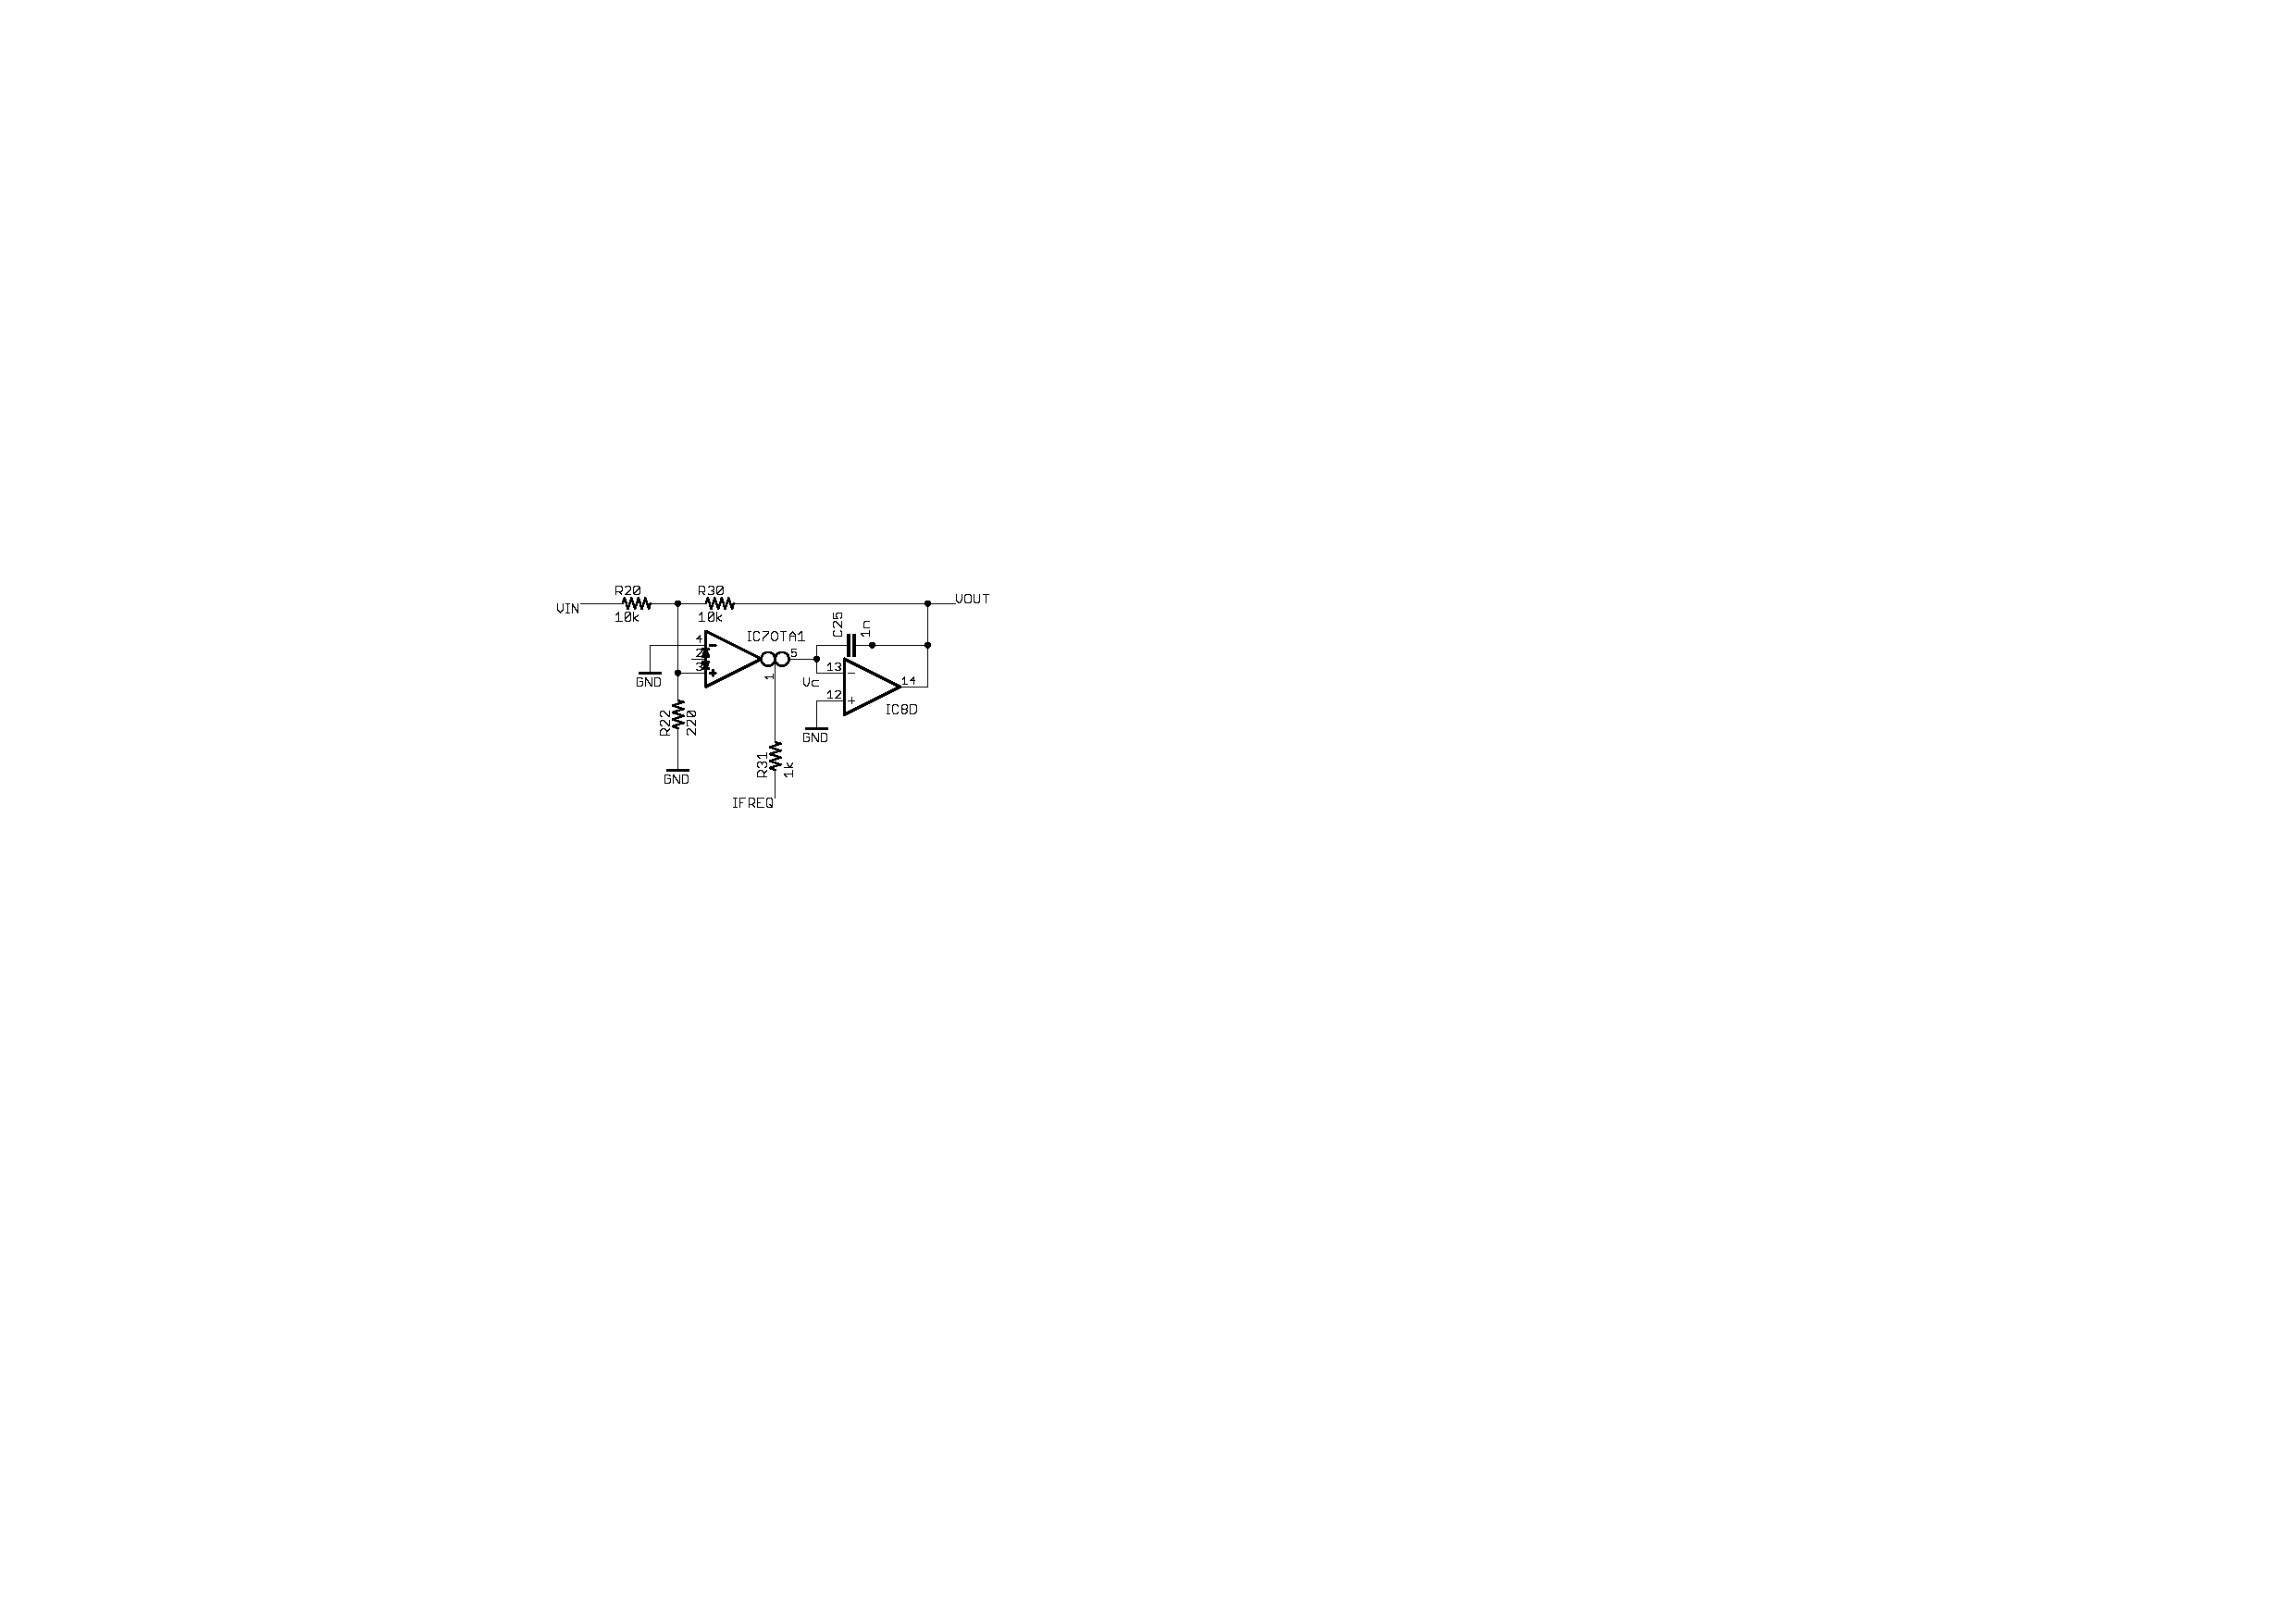
\includegraphics[width=0.8\textwidth]{smr4_otac_cell.pdf}
\caption{OTA-integrator low-pass cell.}
\label{fig:otac}
\end{figure}

Let's start by the OTA. Kirchoff in $V_+$ yields:

\begin{eqnarray}
\frac{1}{R_b}(V_{in}(p) - V_+(p)) + \frac{1}{R_b} (V_{out}(p) - V_+(p)) &=& \frac{1}{R_s} V_+(p) \\
V_+(p) &=& \frac{R_s}{R_b + 2 R_s} (V_{in}(p) + V_{out}(p))
\end{eqnarray}

$V_-$ is simply grounded. The current $I_c(p)$ at the output of the OTA is:

\begin{eqnarray}
I_c(p) &=& g_m (V_+(p) - V_-(p)) \\
 &=& 19.2 I_{freq} \frac{R_s}{R_b + 2 R_s} (V_{in}(p) + V_{out}(p))
\end{eqnarray}

The operational amplifier $IC_{8D}$ is in a simple inverting ``current to voltage" configuration:

\begin{eqnarray}
V_{out}(p) &=& - I_c(p) Z_{feedback}(p) \\
 &=& - \frac{I_c(p)}{Cp} \\
 &=& - 19.2 I_{freq} \frac{R_s}{(R_b + 2 R_s)Cp} (V_{in}(p) + V_{out}(p))
\end{eqnarray}

Solving for $V_{out}(p)$ and dividing by $V_{in}(p)$, we find the transfer function:

\begin{eqnarray}
H(p) &=& \frac{-1}{1 + \frac{(R_b + 2 R_s)}{R_s} Cp \frac{1}{19.2 I_{freq}}}
\end{eqnarray}

The pole is at the frequency $f$ such that:

\begin{eqnarray}
0 &=& 1 + \frac{(R_b + 2 R_s)}{R_s} C 2\pi f \frac{1}{19.2 I_{freq}} \\
f &=& -\frac{19.2 I_{freq}}{2 \pi \frac{(R_b + 2 R_s)}{R_s} C}
\end{eqnarray}

At this stage, we can already pick values for $R_b$, $R_s$, $C$ and design the exponential current source so that its current range translate into a target frequency range using the formula above.

The values that have been chosen for $R_b$, $R_s$ and $C$ follow closely those given in the application schematics of the SSM2040 datasheet (Figure 9 of the datasheet):

\begin{eqnarray*}
R_b &=& 10 k \Omega \\
R_s &=& 220 \Omega \\
C &=& 1 nF
\end{eqnarray*}

$R_s = 200 \Omega$ in the SSM2044 datasheet, but we have privileged here values in the E12 series.

\subsection{Exponential current source}

As we've seen in the previous section, the cutoff frequency is proportional to the biasing current $I_{freq}$ of the OTAs. Since we want to achieve an exponential frequency control, we need to produce a control current which is an exponential function of the input CV. This is achieved by the exponential current source in figure \ref{fig:expo}.

\begin{figure}
\centering
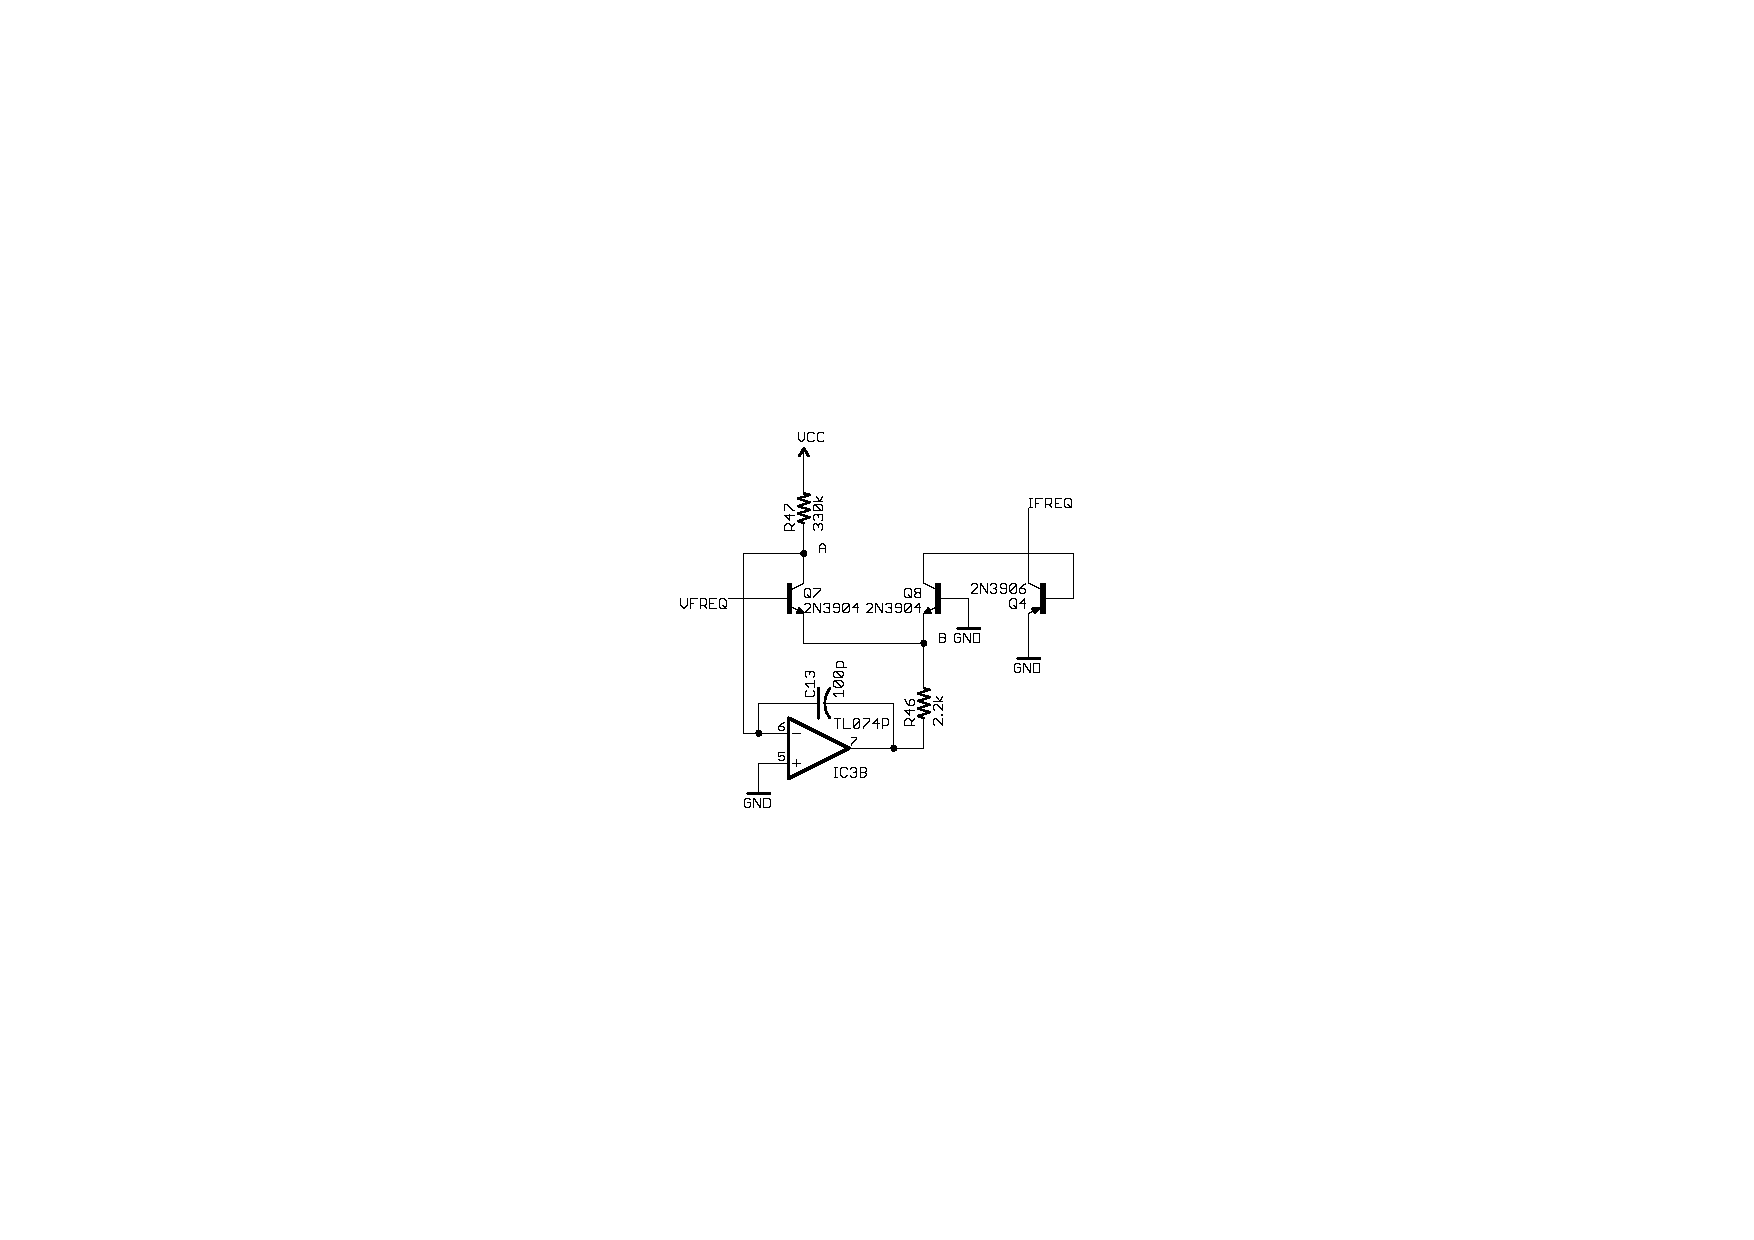
\includegraphics[width=0.6\textwidth]{smr4_expo_current_source.pdf}
\caption{Exponential current source.}
\label{fig:expo}
\end{figure}

Let's start with the core of the circuit -- the NPN transistor pair Q7 and Q8 (we'll see later why NPN instead of PNP). Ebers-Moll for Q7 and Q8 yields the collector currents for both transistors:

\begin{eqnarray}
I_{c7} &=& I_{s7} \left(\exp \left( \frac{V_{be7}}{V_T} \right) - 1 \right) \\
I_{c8} &=& I_{s8} \left(\exp \left( \frac{V_{be8}}{V_T} \right) - 1 \right)
\end{eqnarray}

$V_T$ is the thermal voltage, equal to $26 mV$ at room temperature. We'll see later that $\exp \left( \frac{V_{be7}}{V_T} \right)$ is an order of magnitudes bigger than 1, it is thus a sane approximation to ignore the $- 1$ term. Assuming that the transistor have the same characteristics, $I_{s7} = I_{s8}$. Thus we have, by substituting in the second equation the value of $I_{s8}$ derived from the first one:

\begin{equation}
I_{c8} = I_{c7} \exp \left( \frac{V_{be8} - V_{be7}}{V_T} \right)
\end{equation}

Since the base of $Q8$ is grounded, and since the emitter of $Q7$ and $Q8$ are at the same potential:

\begin{equation}
I_{c8} = I_{c7} \exp \left( -\frac{V_{freq}}{V_T} \right)
\end{equation}

The value of $I_{c8}$ is simply:

\begin{equation}
I_{c8} = \frac{V_{cc} - V_a}{R_{47}} = \frac{V_{cc}}{R_{47}}
\end{equation}

$V_a$ is null because the point $A$ is virtually grounded. Indeed, the whole point of the operational amplifier $IC_{3B}$ is to keep the point $A$ at a constant potential. $C_{13}$ is only here to stabilize the op-amp. $R_{46}$ works as a current limiter -- we can compute its value later to make sure that the maximum current $I_{c8}$ translates into a reasonable frequency.

Note that the biasing current $I_{c8}$ varies in the inverse direction of $V_{freq}$~-- when $V_{freq}$ increases, $I_{c8}$ decreases. This is not a problem because $V_{freq}$ is generated by an op-amp in an inverting configuration.

This brings us to discuss the roles of $Q4$ (and $Q3$, $Q5$, $Q6$). If $I_{c8}$ was directly used as a biasing current for the OTA, the circuit wouldn't work at all, because the biasing current pin of the LM13700 is not ``pointing" in the right direction. A way of avoiding this problem would be to simply replace $Q_7$ and $Q_8$ by PNP ; but if we do so, $I_{c8}$ varies in the same direction as $V_{freq}$, and this means that the CV-scaling stage described in the next section should not invert the input signal. This leaves 3 options:

\begin{itemize}
\item Design the CV-scaling stage as a non-inverting summer. This doesn't work well because the op-amp in such a non-inverting configuration has a gain above $1$, while the scaling we want to achieve requires a gain lower than $1$. You can also observe that the input voltage being in the $0-5V$ range ; and the op-amps being powered by $\pm 5V$, using a circuit with a gain above 1 will result in clipping.
\item Add a simple inverting amplifier with a gain of 1 at the output of the (inverting) summer ; or more generally design the CV-scaling circuit with two inverting stages. This is an option frequently seen (e.g. Polyfusion) ; but the constraints on the board size made it impractical.
\item Use an entirely passive CV-scaling circuit, with $V_{freq}$ being the summing node. This solution has also been seen in a couple of circuits erring on the minimalistic side (e.g. EFM wildcat, VCF 1 and 2). The main reason why this solution was rejected is that the Shruthi-1 generates PWM control signals, which need to be filtered -- so the CV-scaling stage also needs to have a low-pass filter. The ``no-summing op-amp" approach requires the use of a passive filter, which, in our experiments poured too much high-frequency noise on the ground.
\end{itemize}

None of those solutions being particularly appealing\footnote{There seems to be a fourth solution we have not verified, and which requires no extra inversion~-- use PNPs, ground the base of $Q7$ and apply the control voltage to the base of $Q8$.}, we decided to stick to NPNs for the core exponential converters, and then use PNPs to ``replicate" the generated current, with the right direction. The circuit thus uses 2 NPN for the core exponential converter, and 1 PNP per pole, instead of 1 PNP for the core exponential converter and 1 PNP per pole. This extra transistor proved to be easier to lay out and cheaper than an extra TL071.

One thing not discussed here is temperature compensation. While the main temperature dependent factors (saturation currents) have been neutralized by the ``resistor pair" design (as long as the transistors are matched and thermically coupled), there remains a temperature dependent term, $V_T$. This term is not compensated. A rough estimate of the variation in frequency is less than $\pm 10\%$ for a change in temperature of $\pm 5^oC$~-- not good for a VCO, but ok-ish for a VCF.

\subsection{CV scaling}

The CV scaling stage is fed with a 0/5V PWM signal generated by the microcontroller, and generates a scaled voltage which will translate into an appropriate cutoff frequency range. In addition to the scaling itself, it also actively smoothes the high-frequency PWM control signal into a near-DC voltage. Its schematics is given in figure \ref{fig:cvscale}.

\begin{figure}
\centering
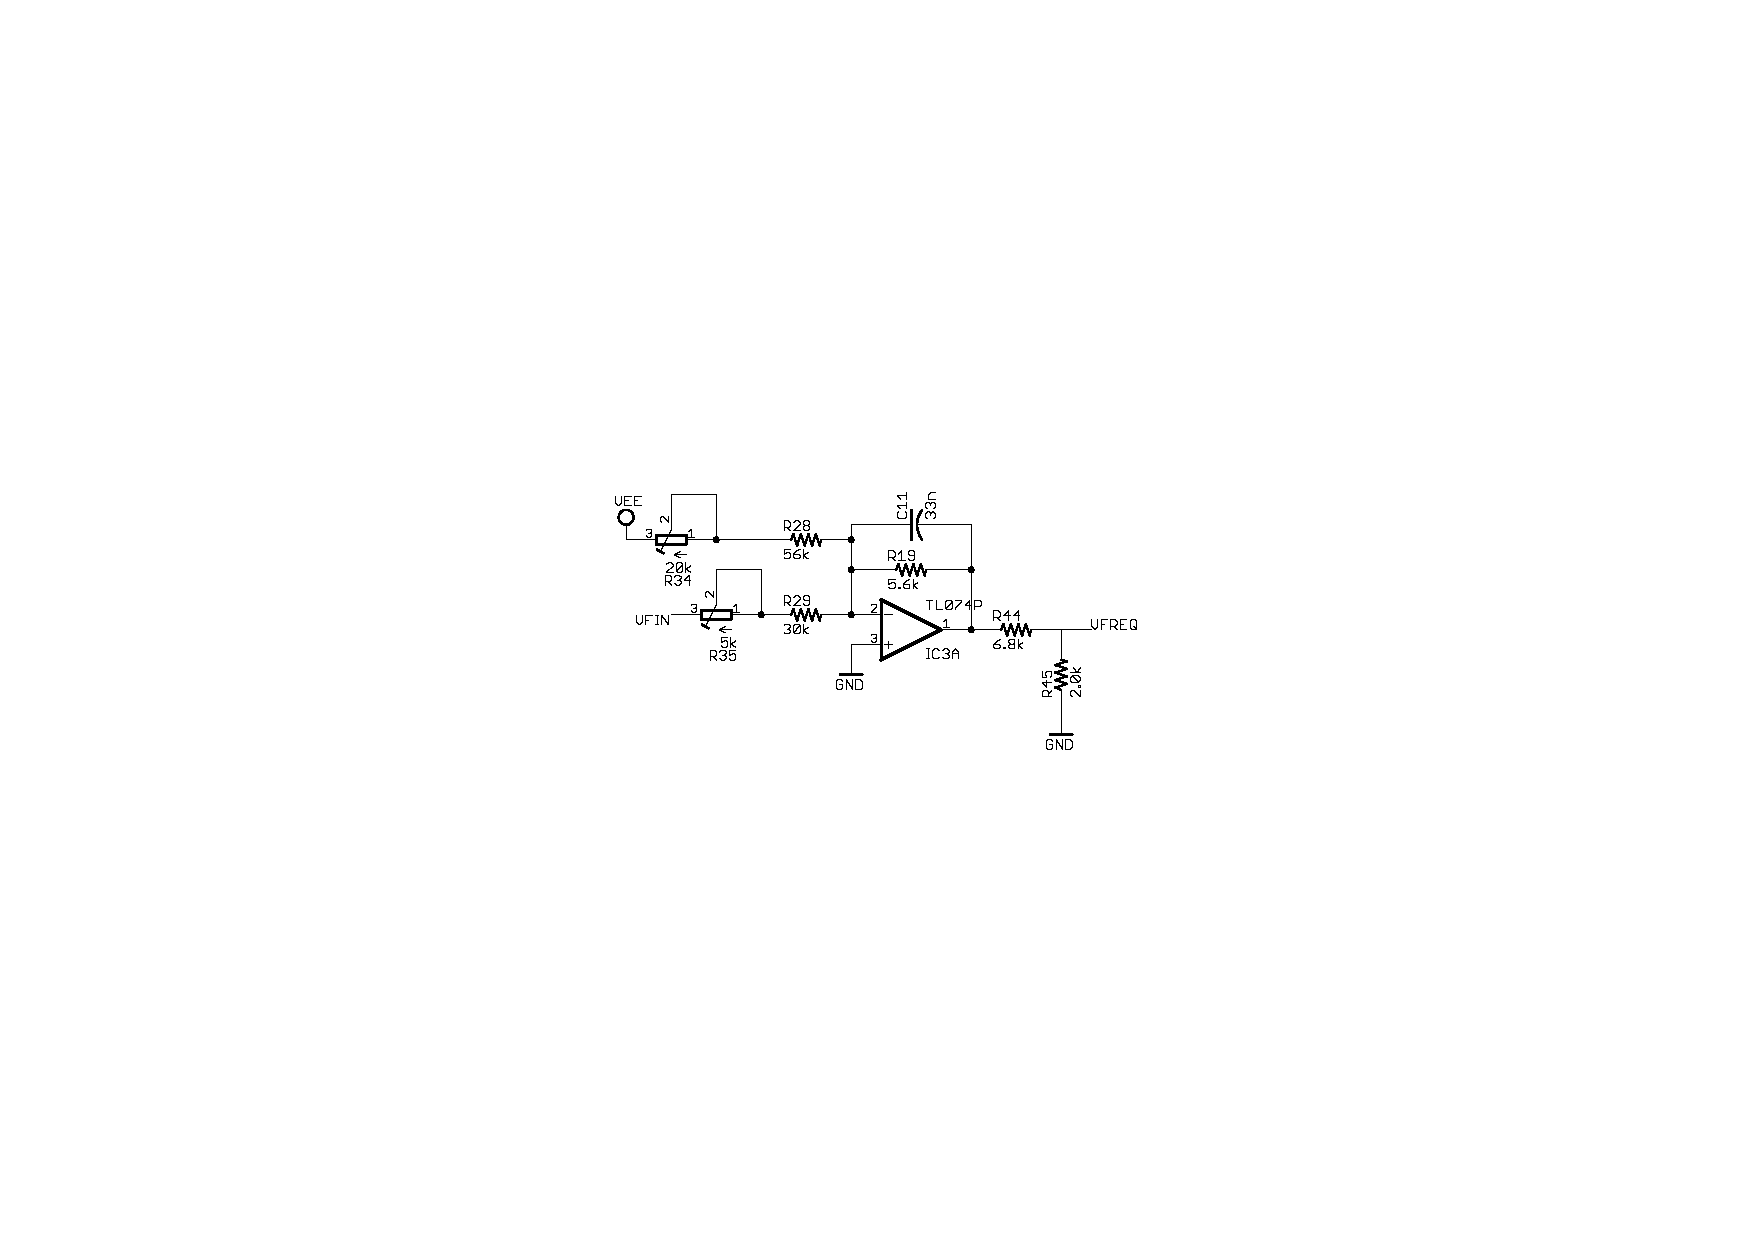
\includegraphics[width=0.8\textwidth]{smr4_scaling.pdf}
\caption{CV-scaling.}
\label{fig:cvscale}
\end{figure}

The voltage at the output of the op-amp is given by:

\begin{equation}
V_o(p) = -\frac{R_{19}}{R_{28} + R_{34}} V_{ee} -\frac{Z_f(p)}{R_{29} + R_{35}} V_{fin}(p)
\end{equation}

Where $Z_f(p)$ is the equivalent impedance of the feedback loop, consisting of $R_{19}$ in parallel with $C_{11}$. Note that in the first term, this impedance is simply $R_{19}$ since a capacitor in parallel with a resistor has no effect on DC currents. In the second term, it is equal to:

\begin{equation}
Z_f(p) = \frac{R_{19}}{1 + R_{19}C_{11}p}
\end{equation}

Thus, the cutoff frequency of the filter smoothing the PWM control signals is $\frac{1}{2 \pi R_{19}C_{11}} = 861.7 Hz$ with values given on the schematics. This means that the PWM carrier is attenuated by $6\log_2 \frac{39062}{861.7} = 33dB$. Given this (moderately) high attenuation factor, it is safe to consider that when the cutoff value is constant, the circuit behaves as if $V_{fin}$ is a pure DC component in the $[0, 5]V$ range instead of a PWM signal.

Adding the contribution of the voltage divider comprised of $R_{44}$ and $R_{45}$, we find:

\begin{equation}
V_{freq} = \frac{R_{45}}{R_{45} + R_{44}} \left(-\frac{R_{19}}{R_{28} + R_{34}} V_{ee} -\frac{R_{19}}{R_{29} + R_{35}} V_{fin}\right)
\end{equation}

\subsection{Component values}

\subsubsection{Constraints}

How are the different values of the component selected? From the past sections, some characteristics of the ICs used in the circuit, and some common sense, we can gather a set of constraints ($\sim$ denotes an order of magnitude in this section) the component values must satisfy:

\paragraph{Input impedance} The input impedance of the CV scaling circuit $R_{35} + R_{29}$ shouldn't be too low, at least $\sim 10k \Omega$.

\paragraph{OTA small voltage constraint} The signal at the input of the OTA should not exceed $\sim 10mV pp$.

\paragraph{OTA small biasing current constraint} The biasing current of the OTA should not exceed $\sim 1mA$.

\paragraph{Cutoff frequency constraint} The frequency range of the filter must span the audible spectrum ($20 Hz$ to $20kHz$), and it should be easy to ``tune" it to the fundamental frequency of the oscillators. To this effect, we have decided to eschew the $1 V/octave$ standard (which would have given a very narrow frequency range given that the input signal is in the $[0, 5]V$ range, and to use another approach.

By default (in the ``init" patch), the Shruthi-1 patches the ``note" modulation source to the ``cutoff" modulation destination, with an amount of 63 corresponding to an (almost) unitary modulation. In other words, if the base cutoff setting of the Shruthi-1 is set to $n$, the PWM control signal corresponds to a smoothed DC voltage of:

\begin{equation}
V_{fin} = V_{cc} \frac{n + \mbox{Midi note number} - 64}{128}
\end{equation}

From this, it appears that if we want a 1:1 tracking of the filter frequency to the fundamental frequency of the oscillators, the cutoff frequency should be multiplied by a semitone ($2^\frac{1}{12}$) every time the Midi note number is increased by $1$, that is to say everytime $V_{fin}$ steps by a $\frac{5}{128}$ increment. This yields the rather odd scale of $0.46875V.oct^{-1}$, which is the target $V.oct^{-1}$ scale of the filter.

The filter is thus expected to cover a range of $\frac{128}{12} = 10.66$ octaves~-- the highest cutoff value will be 1625 the lowest cutoff value. The $12.3 Hz$ -- $20kHz$ range has this exact ratio, spans the audible range, and is, incidentally, exactly one fifth above the range of the notes described by the MIDI standard (the lowest note has a fundamental frequency of $8.18 Hz$. One fifth above: $12.27 Hz$).

\paragraph{Pragmatic constraints} Resistor values should be preferably in the E12 series ; and the number of distinct component values should be minimized.

How to find a solution meeting all these constraints? We went the nerdy way and used a constraint solver (implemented in Python, hopefully, to be released later) to search for sets of solutions matching these constraints.

We provide in the rest of this section a validation of the selected values.

\subsubsection{Validation}

\paragraph{Input impedance} Greater than $30k\Omega$, all good!

\paragraph{OTA small voltage constraint} The signal output by the digital oscillator is in the $0-5V$ range, then AC-coupled and scaled by a gain of $0.33$ in the input mixer. The signal at the input of the OTA-C cells has thus a range of $\frac{R_s}{R_b + R_s} \times 0.33 \times 5 = 35mV$.

\paragraph{OTA small current constraint} The worst case corresponds to the maximum cutoff value, which can be obtained with an input signal $V_{fin} = 5V$, $R_{35}$ trimmed to 0, and $R_{34}$ trimmed to $20k\Omega$. In this case, $V_{freq} = 128mV$ and $I_{freq} = 2mA$, small enough to avoid destroying the LM13700.

\paragraph{Frequency range} Let us check first that the lowest cutoff frequency attainable with the filter is in the expected range. $V_{fin}$ is set to $0V$. Depending on how $R_{34}$ is trimmed, we have:

\begin{eqnarray}
-113mV \leq &V_{freq}& \leq -83mV \\
0.19\mu A \leq &I_{freq}& \leq 0.60\mu A \\
12Hz \leq &f& \leq 39Hz
\end{eqnarray}

The target lowest frequency is attained exactly when the trimmer is at its zero position. Keeping this trimmer setting, let us check what is the maximum cutoff frequency that can be reached. $V_{fin}$ is now set to $5V$. Depending on how $R_{35}$ is trimmed, we have:

\begin{eqnarray}
68mV \leq &V_{freq}& \leq 98mV \\
0.208 mA \leq &I_{freq}& \leq 0.669 mA \\
13.3kHz \leq &f& \leq 43.1kHz
\end{eqnarray}

The target frequency range is thus feasible. Now there's a secret: from a pure theoretical point of view, one can get away with the trimmers and replace $R_{29}$ by a $33k\Omega$ resistor (nice value!)~-- which is the original solution the constraint solver yielded~-- and one will find a theoretical frequency range of $12.3 Hz$ to $20.5kHz$, which is dead on. Things did not turn that well in reality due to the wild tolerances of capacitors, and (possibly) the fact that the transistors were not matched. For this reason only, trimmers were added.

\section{VCA and resonance feedback loop}
\label{sec:vca}

TODO

\section{Future work}

\begin{itemize}
\item Stricter temperature compensation on the exponential converter.
\item Try the ``PNP + swapped $Q7$/$Q8$" trick to avoid the extra transistors in the exponential converter.
\end{itemize}

\end{document}
